\chapter{Literature Notes and Commentary}

\section{Differential Sharpe Ratio}

\cite{drl_mvo} utilizes the Differential Sharpe Ratio to implement and evaluate a reinforcement learning agent.
The Differential Sharpe Ratio is based on Portfolio Management Theory, and is developed in the author' previous works \cite{diff_sharpe_ratio_paper} and \cite{diff_sharpe_ratio_book}.
We briefly review the theory developed in both sources.

The traditional definition of the Sharpe Ratio is the ratio of expected excess returns to volatility.
If $R_t$ is the return of the portfolio at time $t$, and $r_f$ is the risk-free rate then
\begin{align*}
  \mathcal{S} = \frac{\mathbb{E}_t[R_t] - r_f}{\sqrt{\Var_t[R_t]}}
\end{align*}

This works well to analyze a strategy once all data is collected.
The goal of traditional portfolio theory is to maximize the Sharpe Ratio over the given time period (equivalently,
to maximize the mean-variance utility function).

Unfortunately, this will not work for a reinforcement learning agent. The agent must be given a reward after every time step,
but the traditional Sharpe ratio is only calculated at the end.

The Differential Sharpe Ratio attempts to remedy this by approximating a change in the total Sharpe ratio up to that point.
By summing together many of these incremental changes (though approximate), the cumulative rewards is an approximation of the total
Sharpe ratio over the complete time period.

The approximation works by updating moment-based estimators of the expectation and variance in the Sharpe Ratio formula.
Let $A_t$ and $B_t$ be estimates of the first and second moments of the return $R_t$ up to time $t$.
After time step $t$, having obtained $R_t$, we perform the following updates:
\begin{align*}
  \Delta A_t = R_t - A_{t-1} && A_t = A_{t-1} + \eta \Delta A_t \\
  \Delta B_t = R_t - B_{t-1} && B_t = B_{t-1} + \eta \Delta B_t
\end{align*}
where $A_0 = B_0 = 0$ and $\eta \sim 1/T$ is an update parameter, where there are $T$ total time periods.
These updates are essentially exponential moving averages.

Let $S_t$ be an approximation of the Sharpe Ratio up to time $t$ based on estimates $A$ and $B$. That is,
\begin{align*}
  S_t = \frac{A_t}{\sqrt{B_t - A_t^2}}
\end{align*}
The definition here ignores the risk-free rate term. $K_\eta$ is a normalization constant to ensure an unbiased estimator.

Pretend that at the update for time $t$, $A_{t-1}$ and $B_{t-1}$ are constants,
and $R_t$ is also a known constant. Then the updates to $A_t$ and $B_t$ really only depend on the time step parameter $\eta$.
Indeed, if $\eta = 0$, then $A_t = A_{t-1}$ and $B_t = B_{t-1}$, so $S_t = S_{t-1}$.
Now consider varying $\eta$; expanding the Sharpe ratio estimator formula in Taylor series gives
\begin{align*}
  S_t \approx S_{t-1} + \eta \frac{\diff S_t}{\diff \eta}\Big|_{\eta = 0} + o(\eta^2)
\end{align*}

If $\eta$ is small, the final term is negligible, so this formula gives us an exponential-moving-average update for $S_t$.
The Differential Sharpe Ratio is defined to be proportional derivative in that expression. With some tedious calculus, we find that
\begin{align*}
  D_t &= \frac{\diff S_t}{\diff \eta} = \frac{\diff}{\diff\eta}\left[ \frac{A_t}{\sqrt{B_t - A_t^2}} \right] = \frac{\frac{\diff A_t}{\diff \eta} \sqrt{B_t - A_t^2} - A_t \frac{\frac{\diff B_t}{\diff \eta} - 2 A_t \frac{\diff A_t}{\diff \eta}}{2 \sqrt{B_t - A_t^2}}}{B_t - A_t^2} \\
  &= \frac{\Delta A_t \sqrt{B_t - A_t^2} - A_t \frac{\Delta B_t - 2 A_t \Delta A_t}{2 \sqrt{B_t - A_t^2}}}{B_t - A_t^2}
  = \frac{B_t \Delta A_t - \frac{1}{2} A_t \Delta B_t}{(B_t - A_t^2)^{3/2}}
\end{align*}

This reward function is simple to implement in an environment. The authors of the original papers provide
experimental support for the value of this reward function in a reinforcement learning setting.




\section{Transaction Costs}

\cite{drl_framework} contains an excellent walkthrough of the mathematics for modeling transaction costs
in RL environment updates. We provide a shortened version here.

Suppose we have $m$ tradeable assets and the risk-free asset. Let $\mathbf v_t = (1, v_{1,t}, v_{2,t}, \ldots v_{m,t}) \in \R^{m+1}$ be the
prices of the assets at time $t$ (the first entry is the risk-free asset). The raw return vector is defined as
$\mathbf y_t = \mathbf v_t \varoslash \mathbf v_{t-1} \in \R^{m+1}$, where division is element-wise. Suppose the portfolio
weight vector during time period $t$ is $\mathbf w_t \in \R^{m+1}$, and let the value of the portfolio value at time $t$ be $p_t$.
If we were not considering transaction costs, then the portfolio return would be $\frac{p_t}{p_{t-1}} = \mathbf y_t \cdot \mathbf w_t$.

Unfortunately, buying and selling assets incurs transaction costs. Let $\mathbf w_t' \in \R^{m+1}$ be the effective portfoliio weights
at the end of time $t$ (it has changed from $\mathbf w_t$ due to the changes in price). We have
\begin{align*}
  \mathbf w_t' = \frac{\mathbf y_t \odot \mathbf w_t}{\mathbf y_t \cdot \mathbf w_t}
\end{align*}
where $\odot$ is element-wise multiplication. Between time $t-1$ and time $t$, the portfolio value is also
adjusted from $p_{t-1} \in \R$ to $p_t' = p_{t-1} \mathbf y_t \cdot \mathbf w_{t-1}$. Let $p_t$ be the value of the portfolio
after transaction costs, and let $\mu_t \in \R$ be the transaction cost factor, such that $p_t = \mu_t p_t'$.
We can keep track of the relevant time of each variable with the following diagram:

\begin{center}
  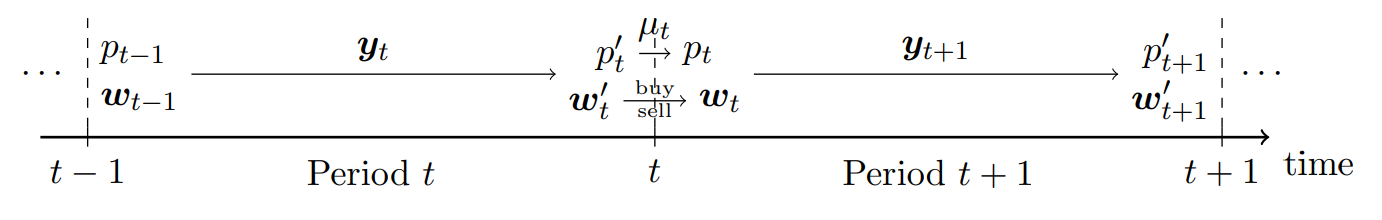
\includegraphics[width=13cm]{transaction_cost_time_updates.png}
\end{center}

In this paradigm, the final portfolio value at time $T$ is
\begin{align*}
  p_T = p_0 \prod_{t=1}^T \frac{p_t}{p_{t-1}} = p_0 \prod_{t=1}^T \mu_t \mathbf y_t \cdot \mathbf w_{t-1}
\end{align*}
The main difficulty is in determining the factor $\mu_t$, since it is an aggregate of all the transaction cost penalties.

Let $c_s \in [0, 1)$ be the commission rate for selling. We need to sell some amount of asset $i$ if 
there is more of asset $i$ in $\mathbf w_t'$ than in $\mathbf w_t$ by dollar value. Mathematically, this condition
is $p_t' w_{i,t}' > p_t w_{t,i}$, which is equivalent to $w_{i,t}' > \mu_t w_{i,t}$. Thus, the total amount of
money raised from selling assets is
\begin{align*}
  (1-c_s) p_t' \sum_{i=1}^m (w_{i,t}' - \mu_t w_{i,t})^+
\end{align*}
where $(\cdot)^+ = \max\{0, \cdot\} = \mathrm{ReLU}(\cdot)$. This money, as well as the money from adjusting the cash reserve
from $p_t' w_{0,t}'$ to $p_t w_{0,t}$, is used to purchase assets according to the opposite condition.
Let $c_p \in [0, 1)$ be the commision rate for purchasing. Equating the amount of money available from selling/cash and the amount of money
used for purchasing assets yields
\begin{align*}
  (1-c_p)\left[ w_{0,t}' - mu_t w_{0,t} + (1-c_s) p_t' \sum_{i=1}^m (w_{i,t}' - \mu_t w_{i,t})^+ \right] = p_t'\sum_{i=1}^m (\mu_t w_{i,t} - w_{i,t}')+
\end{align*}
Moving terms around and simplifying the ReLU expressions, we find that $\mu_t$ is a fixed-point of the function $f$ defined as:
\begin{align*}
  \mu_t = f(\mu_t) = \frac{1}{1 - c_p w_{0,t}}\left[ 1 - c_p w_{0,t}' - (c_s + c_p - c_s c_p) \sum_{i=1}^m (w_{i,t}' - \mu_t w_{i,t})^+ \right]
\end{align*}
$f$ is a nonlinear function. However, for reasonable values of $c_s and c_p$, $f$ is both monotone increasing and a contraction, so its unique fixed point
can be found by iteratively computing values of $f$. This procedure is fairly efficient and easy to implement.
